% This template was partially made with assistance from Microsoft Co-pilot

% ------------------------------------------------------------------
% CAPSTONE SOFTWARE REQUIREMENTS SPECIFICATION (SRS)

% 
% This template is inspired by IEEE 29148 but simplified for use in 
% a senior software engineering capstone project. 
% 
% The goal is not to maximize document length. 
% The goal is to produce a clear, testable, and traceable set of 
% requirements that can guide design, implementation, and testing. 
% 
% Recommended workflow: 
% Stakeholder Requirements 
% -> 
% Use Cases 
% -> 
% Functional Requirements 
% -> 
% Acceptance Tests (will be in your VnV plan)
% -> 
% Traceability Matrix (will excluded traceability for tests, that will be in the VnV plan)
% 
% Students should update this document throughout the project. 
% ------------------------------------------------------------------

\documentclass[12pt]{article}

\usepackage{amsmath, mathtools}
\usepackage{amsfonts}
\usepackage{amssymb}
\usepackage{graphicx}
\usepackage{colortbl}
\usepackage{xr}
\usepackage{hyperref}
\usepackage{longtable}
\usepackage{xfrac}
\usepackage{tabularx}
\usepackage{float}
\usepackage{siunitx}
\usepackage{booktabs}
\usepackage{caption}
\usepackage{pdflscape}
\usepackage{afterpage}

\usepackage[round]{natbib}

%\usepackage{refcheck}

\hypersetup{
    bookmarks=true,         % show bookmarks bar?
      colorlinks=true,       % false: boxed links; true: colored links
    linkcolor=red,          % color of internal links (change box color with linkbordercolor)
    citecolor=green,        % color of links to bibliography
    filecolor=magenta,      % color of file links
    urlcolor=cyan           % color of external links
}

\input{../Comments.text}
\input{../Common.text}

% Used so that cross-references have a meaningful prefix

\newcounter{srnum} %Stakeholder Requirement (SR) Number
\newcommand{\srthesrnum}{SR\thesrnum}
\newcommand{\srref}[1]{SR\ref{#1}}

\newcounter{ucnum} %Use Case (UC) Number
\newcommand{\uctheucnum}{UC\theucnum}
\newcommand{\ucref}[1]{UC\ref{#1}}

\newcounter{reqnum} %Functional Requirement (FR) Number
\newcommand{\rthereqnum}{FR\thereqnum}
\newcommand{\rref}[1]{FR\ref{#1}}

\newcounter{nfrnum} %Non-Functional Requirement (NFR) Number
\newcommand{\rthenfrnum}{NFR\thenfrnum}
\newcommand{\nfrref}[1]{NFR\ref{#1}}

\newcounter{lcnum} %Likely Change (LC) Number
\newcommand{\lthelcnum}{LC\thelcnum}
\newcommand{\lcref}[1]{LC\ref{#1}}

\usepackage{fullpage}

\begin{document}

\title{Software Requirements Specification for \progname: subtitle describing software} 
\author{\authname}
\date{\today}
	
\maketitle

~\newpage

\pagenumbering{roman}

\tableofcontents

~\newpage

\section*{Revision History}

\begin{tabularx}{\textwidth}{p{3cm}p{2cm}X}
\toprule {\bf Date} & {\bf Version} & {\bf Notes}\\
\midrule
14-10-2026 & 1.0 & Added Sections\\
Date 2 & 1.1 & Notes\\
\bottomrule
\end{tabularx}

~\\
\plt{All capstone SRS documents should have a reflection appendix.}

\newpage

\pagenumbering{arabic}

\plt{This SRS template is based on the IEEE template, with input from co-pilot
  and S. Smith. It will get you started.  You should not modify the section
  headings, without first discussing the change with the course instructor.
  Modification means you are not following the template, which loses some of the
  advantage of a template, especially standardization.}

\plt{Feel free to change the appearance of the report by modifying the LaTeX
  commands.}

\plt{This template document assumes that a single program is being documented.
  If you are documenting a family of models, you should start with a commonality
  analysis.}

\plt{The SRS is not generally written, or read, sequentially.  The SRS is a
  reference document.  It is generally read in an ad hoc order, as the need
  arises.}

\plt{Guiding principles for the SRS document:
\begin{itemize}
\item Do not repeat the same information at the same abstraction level.  If
  information is repeated, the repetition should be at a different abstraction
  level.
\end{itemize}
}

\plt{The template description comments should be disabled before submitting this
  document for grading.}

\plt{You can borrow any wording from the text given in the template.  It is part
  of the template, and not considered an instance of academic integrity.  Of
  course, you need to cite the source of the template.}

\plt{When the documentation is done, it should be possible to trace back to the
  source of every piece of information.  Some information will come from
  external sources, like terminology.}

\plt{An SRS document should have the following qualities: unambiguous,
  consistent, complete, validatable, abstract and traceable.}

\plt{The overall goal of the SRS is that someone can learn,
  understand and verify the captured domain knowledge.  They should not have to
  trust the authors of the SRS on any statements.  They should be able to
  independently verify/derive every statement made.}

% ============================================================== 
\section{Introduction} 
% ==============================================================

\plt{Explain what system is being specified. State purpose, users, and project goals.}

\plt{Introduce the name of your software as \progname{}.  Using \progname{} as
a command lets you change the name if necessary and have the change propagate to
all documents.}

\plt{Include a reference to the template this work is based on.  \citet{ISOIECIEEE29148_2018}
justifies the SRS structure and \citet{ISOIECIEEE15288_2023} provides the
broader life-cycle context that underlines modern requirements engineering
practice.}

\subsection{Purpose}

\plt{State the purpose of the system.}

\plt{The purpose should be in the context of the project itself, not in the
  context of this course. Although the ``purpose'' of the document is to get a
  grade, you should not mention this.  Instead, ``fake it'' as if this is a real
  project.}

\progname{} is intended to solve ... \plt{What problem does your program solve?
The description here should be in the problem space, not the solution space.}

\subsection{Scope}
\plt{Briefly describe:
\begin{itemize}
  \item Problem being solved
  \item Intended users
  \item Major functionality
  \item Expected benefits
  \item Clarifying the scope often means saying what the software doesn't do
\end{itemize}
}

\plt{The scope section is relevant for understanding the boundaries of the system. It is also relevant for later determining typical values of inputs. The scope should make it clear what inputs are reasonable to expect. This is a distinction between scope and context (context is a later section).  Scope affects the inputs while context affects how the software will be used.}

TODO

\subsection{Stakeholders}
\begin{itemize}
\item Customer
\item End Users
\item Project Sponsor
\item Development Team
\item Administrators
\end{itemize}

\subsection{Definitions and Acronyms}

\begin{longtable}{p{0.25\textwidth} p{0.65\textwidth}}
\toprule
Term & Definition\\
\midrule
MERLS & A web platform for Mandarin-English child language assessment. It brings together the assessment tools clinicians need, so they can complete their entire workflow in one place.\\
\midrule
BeViz & Software that organizes and visualizes assessment results. It also detects potential interfering behaviors during an assessment (such as parent prompting) so clinicians can review them.\\
\midrule
SAFA & Stands for “Speech Annotation For Application, Access, Accuracy.” It automatically generates transcripts from recorded online speech assessments. Clinicians can then review, verify, and annotate the transcripts.\\
\midrule
Clinician & A direct user of the system, typically an SLP (speech-language pathologist). Each clinician cares for one or more patients. Clinicians review assessment recordings, verify transcriptions and assessment results, and analyze overall performance.\\
\midrule
Patient & An individual who uses MERLS to complete online speech assessments from home. Each patient is assigned to a clinician who oversees their care. Patients can also be referred to as clients.\\
\midrule
Report & A detailed breakdown of a patient’s results for a single speech assessment completed on the MERLS platform.\\
\midrule
Speech Language Pathologist & They can also be referred to as a speech clinician. \\
\midrule
Health Insurance Portability and Accountability Act & An American federal law that permits the use of sensitive patient health information while protecting their privacy \citep{CDC_HIPAA_1996}.\\
\midrule
Finite State Machine & A mathematical model that represents a sequential workflow as a set of states and transitions between them. A state may have one or more transitions leading to different states, which allows for multiple pathways through the workflow. At any given moment, the workflow is in exactly one state and may move to another state through a defined transition.\\
\midrule
SLP & Speech-Language Pathologist\\
\midrule
HCI & Human-Computer Interface\\
\midrule
HCD & Human-Centered Design\\
\midrule
FR & Functional Requirement\\
\midrule
NFR & Non-Functional Requirement\\
\midrule
HIPAA & Health Insurance Portability and Accountability Act\\
\bottomrule
\caption{Definitions and Acronyms} \label{tab:DefinitionsAndAcronyms}
\end{longtable}

\subsection{Characteristics of Intended Reader} \label{sec_IntendedReader}

\plt{This section summarizes the skills and knowledge of the readers of the
  SRS.  It does NOT have the same purpose as the ``User Characteristics''
  section (Section~\ref{SecUserCharacteristics}).  The intended readers are the
  people that will read, review and maintain the SRS.  They are the people that
  will conceivably design the software that is intended to meet the
  requirements.  The user, on the other hand, is the person that uses the
  software that is built.  They may never read this SRS document.  Of course,
  the same person could be a ``user'' and an ``intended reader.''}

\plt{The intended reader characteristics should be written as unambiguously and
  as specifically as possible.  Rather than say, the user should have an
  understanding of physics, say what kind of physics and at what level.  For
  instance, is high school physics adequate, or should the reader have had a
  graduate course on advanced quantum mechanics?}

% ============================================================== 
\section{System Overview}

This section provides general information about the system.  It identifies the
problem, the vision, and the interfaces between the system and its environment.
This section also describes user characteristics and lists the system
constraints.

\plt{The purpose of this section is to provide general information about the
  system so that the specific requirements in the later sections will be easier to
  understand. The general system description section is designed to be
  changeable independent of changes to the functional requirements documented in
  the specific system description. The general system description provides a
  context for a family of related models.  The general description can stay the
  same, while specific details are changed between family members.}

\subsection{Problem Statement}

\plt{Current situation, problem, impact, desired improvement.  You will likely borrow some text from your problem description document.}

TODO

\subsection{Product Vision}

The purpose of this product is to give speech clinicians a single, centralized telehealth platform for reviewing, annotating, and analyzing speech assessments of bilingual children. 
By integrating SAFA’s annotation tools into the platform and incorporating patient records in one place, the product aims to make the assessment analysis process faster, simpler, and easier to use.

\subsubsection{Goals}
\begin{enumerate}
    \item \textbf{Integrate SAFA Into the MERLS platform: }Clinicians should be able to annotate assessments, meaning review and correct the written transcript of a recorded session, without leaving MERLS. SAFA is currently a standalone tool, and bringing it into the platform removes the need to switch between systems.
    \item \textbf{Improve SAFA’s Usability: }The annotation interface should be simple and guided enough that any speech clinician can use it with confidence, regardless of technical background.
    \item \textbf{Speed Up Speech Annotation: }Annotating a bilingual speech assessment should take significantly less time than manual transcription. SAFA has already been shown to reduce annotation time by roughly one-third, and the goal is to preserve or improve on that once SAFA is part of MERLS.
    \item \textbf{Provide a Clinician Record and Analysis Hub: }Clinicians should be able to find a patient’s records and past assessments in a centralized hub. This will simplify clinicians’ workflow, allowing them to quickly reference patient history without navigating multiple disconnected systems.
    \item \textbf{Protect Patient Data: }MERLS handles sensitive health information online; hence the system must keep patient data private and secure. Only authorized clinicians can access a patient’s records, recordings, and assessment results.
\end{enumerate}


  
\subsection{System Context}

\plt{Include users, external systems, APIs, databases, and third-party services.}

\plt{Your system context will include a figure that shows the abstract view of
  the software.  In some cases the diagram will show other external
  entities, besides the user.  For instance, when the software product is a
  library, the user will be another software program, not an actual end user.
  If there are system constraints that the software must work with external
  libraries, these libraries can also be shown on the System Context diagram.
  They should only be named with a specific library name if this is required by
  the system constraint.}

\begin{figure}[h!]
\begin{center}
 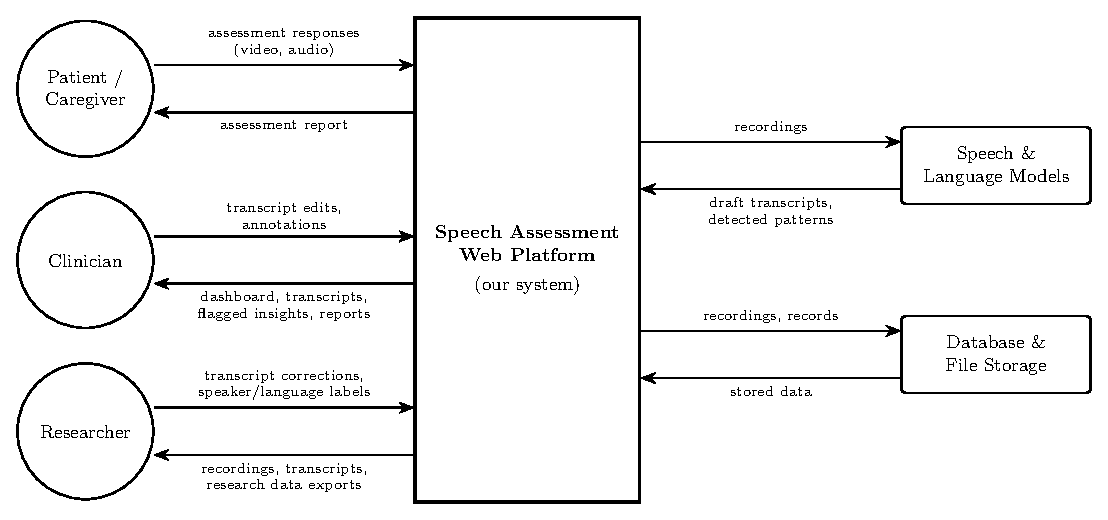
\includegraphics[width=0.6\textwidth]{SystemContextFigure}
\caption{System Context}
\label{Fig_SystemContext} 
\end{center}
\end{figure}

\plt{For each of the entities in the system context diagram its responsibilities
  should be listed.  Whenever possible the system should check for data quality,
  but for some cases the user will need to assume that responsibility.  The list
  of responsibilities should be about the inputs and outputs only, and they
  should be abstract.  Details should not be presented here.  However, the
  information should not be so abstract as to just say ``inputs'' and
  ``outputs''.  A summarizing phrase can be used to characterize the inputs.
  For instance, saying ``material properties'' provides some information, but it
  stays away from the detail of listing every required properties.}

\begin{itemize}
\item User Responsibilities:
\begin{itemize}
\item 
\end{itemize}
\item \progname{} Responsibilities:
\begin{itemize}
\item Detect data type mismatch, such as a string of characters instead of a
  floating point number
\item 
\end{itemize}
\end{itemize}

\plt{Identify in what context the software will typically be used.  Is it for
exploration? education? engineering work? scientific work?. Identify whether it
will be used for mission-critical or safety-critical applications.} 

\plt{This additional context information is needed to determine how much effort
should be devoted to the rationale section.  If the application is
safety-critical, the bar is higher.  This is currently less structured, but
analogous to, the idea to the Automotive Safety Integrity Levels (ASILs) that
McSCert uses in their automotive hazard analyses.}

\subsection{User Characteristics} \label{SecUserCharacteristics}

\plt{This section summarizes the knowledge/skills expected of the user.
  Measuring usability, which is often a required non-function requirement,
  requires knowledge of a typical user.  As mentioned above, the user is a
  different role from the ``intended reader,'' as given in
  Section~\ref{sec_IntendedReader}.  As in Section~\ref{sec_IntendedReader}, the
  user characteristics should be specific an unambiguous.  For instance, ``The
  end user of \progname{} should have an understanding of undergraduate Level 1
  Calculus and Physics.''}

\subsection{System Constraints}

\plt{System constraints differ from other type of requirements because they
  limit the developers' options in the system design and they identify how the
  eventual system must fit into the world. This is the only place in the SRS
  where design decisions can be specified.  That is, the quality requirement for
  abstraction is relaxed here.  However, system constraints should only be
  included if they are truly required.}

\plt{This is where you would mention platform constrains, and licensing
restrictions.}

% ============================================================== 
\section{Stakeholder Requirements}

\plt{Technology-independent requirements.  These come from statements made by
the stakeholders.  You will find these through interviews and surveys.  They are
often expressed in natural language.  They are not necessarily testable, but
they should be verifiable.}

\plt{The stakeholder requirements are numbered so that you can have traceability to other parts of your document.}

\noindent \begin{itemize}

\refstepcounter{srnum}
\item[SR\thesrnum] \label{SR_Label1} TODO

\refstepcounter{srnum}
\item[SR\thesrnum] \label{SR_Label2} TODO

\refstepcounter{srnum}
\item[SR\thesrnum] \label{SR_Label3} TODO

\end{itemize}

\plt{You should give your SRs meaningful labels, so that you can refer to them
in other parts of the SRS.  The label names should be meaningful mnemonics, not
numbers.}

% ============================================================== 
\section{User Personas}

\subsection{Overworked SLP in Favour of Automating the Speech Analysis Process}
\begin{itemize}
\item Name: James Caveat
\item Description: James is a speech clinician at a large hospital, where he is responsible for more than 30 patients. His heavy workload means he must review many speech assessments during his working hours, leaving him little time to carefully absorb and transcribe what he is watching. As a result, it is difficult for him to give each assessment the attention it deserves.
\item Goals: Speed up the analysis of speech assessments, receive assessment results quickly, obtain meaningful and clinically useful insights from each assessment, use a single system rather than learning and switching between multiple software tools, and have one simple place to organize his notes and patient information.
\item Frustrations: James is discouraged by the amount of time it takes to annotate speech data, exhausted by having to watch and listen to numerous assessment recordings from start to finish, struggles to organize assessment data he collects, and has trouble analyzing large amounts of unstructured data.
\item Technical Ability: James is comfortable with the basic tools he uses every day, but he is not technically fluent. He finds it difficult to move between different software systems and prefers to learn one tool well.
\end{itemize}

\subsection{Persona 2}
\begin{itemize}
\item Name:
\item Description:
\item Goals:
\item Frustrations:
\item Technical Ability:
\end{itemize}

% ============================================================== 
\section{Use Cases}
\plt{Use cases are a way to describe the interactions between users and the system.
  They are typically written in natural language and describe the steps that a
  user takes to achieve a specific goal.  Use cases can be used to identify
  functional requirements and to create test cases.}  
\plt{Typically 8-15 substantial use cases.}

\refstepcounter{ucnum} \label{UC_Label4}
\subsection{\ucref{UC_Label4}: Assign Speaker Roles to the Auto-Generated Transcript}

\textbf{Primary Actor}

Clinician, System

\textbf{Preconditions}
\begin{itemize}
\item The clinician must be logged into their account in the system
\item The clinician has selected a patient and opened one of that patient’s video assessments
\end{itemize}

\textbf{Main Success Scenario}
\begin{enumerate}
\item The clinician selects and loads the video assessment they want to analyze 
\item The system auto-generates transcriptions for the video assessment 
\item The system displays the video playback along with the auto-generated transcriptions as chunks of text
\item The clinician selects a chunk 
\item The system indicates which chunk is selected and presents that chunk’s details for editing
\item The clinician selects the “Speaker” dropdown in the chunk’s detail view
\item The system displays the following list of options for different possible speakers
    \begin{itemize}
      \item System
      \item Child
      \item Parent
      \item Experimenter
      \item Multiple Speakers
      \item Others
    \end{itemize}
\item The clinician selects the correct role for the current speaker
\item The system labels the chunk with the selected role
\item The clinician repeats steps 4-9 for the remaining chunks
\end{enumerate}

\textbf{Alternative Flows}
\begin{itemize}
\item[10a.] The clinician may select any segment in any order, and the system indicates the newly selected segment. The clinician can then make any edits to the chunk of text using the given options.
\end{itemize}

\textbf{Postconditions}
\begin{itemize}
\item Each segment the clinician labeled has its assigned speaker role, and the roles are saved with the transcript.
\item The labeled roles are still shown when the clinician reopens the assessment.
\end{itemize}

% ----
\refstepcounter{ucnum} \label{UC_Label5}
\subsection{\ucref{UC_Label5}: Edit and Update Assessment Results}

\textbf{Primary Actor}

Clinician

\textbf{Preconditions}
\begin{itemize}
\item The clinician has an account and is logged in
\item The clinician is analyzing one of their patient’s speech assessments
\end{itemize}

\textbf{Main Success Scenario}
\begin{enumerate}
\item The clinician opens the assessment questions for the assessment
\item The system displays the assessment questions alongside the video of the point in the recording where each question was asked
\item The system indicates which questions have potential interference behavior
\item The clinician selects a flagged question
\item The clinician decides the flag is unjustified and removes it
\item The system saves the change and shows the question without the flag
\item The clinician moves on to another part of the analysis, such as annotating the transcript
\item The clinician notices interference behavior from a parent in a part of the recording they had previously cleared
\item The clinician returns to the affected question
\item The clinician flags the question again and adds a note describing the parent interference
\item The system saves the flag and notes and shows them with the question
\end{enumerate}

\textbf{Alternative Flows}
\begin{itemize}
\item[3a.] The system does not flag a question, but the clinician notices interference while working on another part of the analysis. The clinician returns to that question, flags it, and adds a note.
\item[10a.] The clinician changes their mind again and removes the flag or edits the note. The system saves the update and shows the latest version.
\end{itemize}

\textbf{Postconditions}
\begin{itemize}
\item The question shows the clinician’s latest flag status and notes
\item The latest flag status and notes are included in the generated assessment report.
\end{itemize}

% ----
\refstepcounter{ucnum} \label{UC_Label6}
\subsection{\ucref{UC_Label6}: View Assessment Results and Patient Progress}

\textbf{Primary Actor}

Clinician

\textbf{Preconditions}
\begin{itemize}
\item The clinician has an account and is logged in
\item The clinician has a patient with at least one completed assessment
\end{itemize}

\textbf{Main Success Scenario}
\begin{enumerate}
\item The clinician selects a patient from their list of clients
\item The system displays an overview of the patient, showing their performance trends across attempts and a list of their completed assessments
\item The clinician selects an assessment from the list
\item The system displays a summary of that assessment session, including:
    \begin{itemize}
      \item The date of the assessment
      \item The overall score
      \item The recording of the session
      \item The list of questions asked
    \end{itemize}
\end{enumerate}

\textbf{Alternative Flows}
\begin{itemize}
\item[3a.] The clinician wants to see how the patient’s performance has changed over time. Hence, the clinician reviews the trends shown in the patient overview, where the system presents the patient’s results across multiple attempts.
\end{itemize}

\textbf{Postconditions}
\begin{itemize}
\item The clinician has seen a single assessment’s results as a session summary along with the patient’s progress across different attempts as a trend.
\end{itemize}

\subsection{Use Case Diagrams}
The following use case diagram shows the interactions between the clinician and the system for certain use cases described above. 
\begin{figure}[H]
\begin{center}
 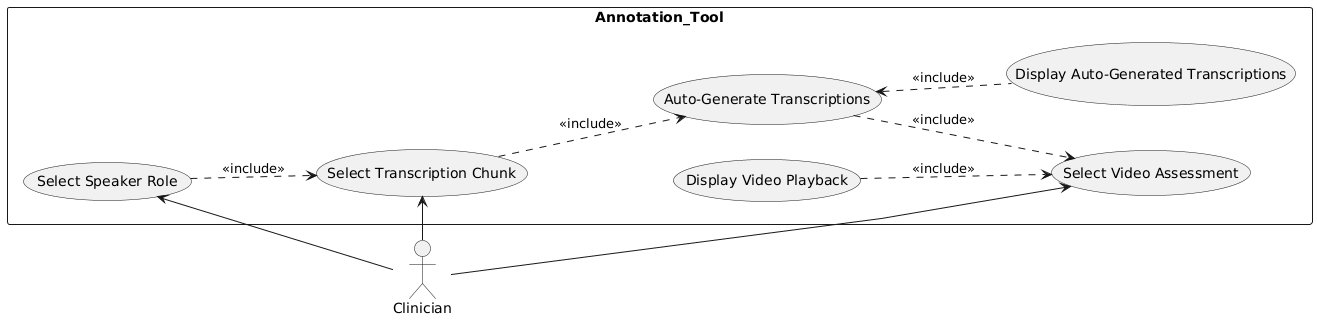
\includegraphics[width=0.75\textwidth]{UC1-Annnotation_Tool.png}
\caption{Use case diagram showing how a clinician assigns speaker roles to an assessment transcript using the annotation tool in MERLS. A detailed description is given in Use Case~\ref{UC_Label4}.}
\label{UC1-Annotation_Tool} 
\end{center}
\end{figure}

% ============================================================== 
\section{Functional Requirements}

\noindent \begin{itemize}

\refstepcounter{reqnum}
\item[\textbf{\rthereqnum} \label{FR_Label1}:] The system shall ...
\\ \textbf{Rationale:}
\\ \textbf{Fit Criterion:}

\refstepcounter{reqnum}
\item[\textbf{\rthereqnum} \label{FR_Label2}:] The system shall ...
\\ \textbf{Rationale:}
\\ \textbf{Fit Criterion:}

\refstepcounter{reqnum}
\item[\textbf{\rthereqnum} \label{FR_Label3}:] The system shall ...
\\ \textbf{Rationale:}
\\ \textbf{Fit Criterion:}

\refstepcounter{reqnum}
\item[\textbf{\rthereqnum} \label{FR_Label4}:]The system shall ...
\\ \textbf{Rationale:}
\\ \textbf{Fit Criterion:}

\refstepcounter{reqnum}
\item[\textbf{\rthereqnum} \label{FR_Label5}:]The system shall ...
\\ \textbf{Rationale:}
\\ \textbf{Fit Criterion:}

\refstepcounter{reqnum}
\item[\textbf{\rthereqnum} \label{FR_Label6}:] The system shall allow clinicians to assign speaker roles and filter assessment transcripts by speaker.
\\ \textbf{Rationale:} Automatically generated transcripts do not identify who is speaking. Clinicians need to distinguish the child’s speech from that of adults, such as the parent or clinician, to analyze the child’s language and identify interfering parent behavior.
\\ \textbf{Fit Criterion:} The system must label every transcript segment from a speaker with the role assigned to that speaker once the clinician assigns it. 

\refstepcounter{reqnum}
\item[\textbf{\rthereqnum} \label{FR_Label7}:] The system shall generate detailed assessment reports from transcriptions, including any edits made by clinicians.
\\ \textbf{Rationale:} Clinicians review and correct the automatically generated transcription, adjust flagged assessment questions, and add notes to individual questions. The report must reflect these changes so that it includes the clinician’s judgment.
\\ \textbf{Fit Criterion:} The system must include any changes made throughout the analysis process made by the clinician, otherwise it outputs the automatically generated content in the report.

\refstepcounter{reqnum}
\item[\textbf{\rthereqnum} \label{FR_Label8}:] The system shall allow clinicians to edit and update assessment results at any time.
\\ \textbf{Rationale:} Clinicians do not always analyze assessments sequentially. They may notice an error in a result or change their judgment after reviewing more of the recording, so they need to be able to go back and change results at any stage. 
\\ \textbf{Fit Criterion:} The system must display the updated result once the clinician submits a change. 

\refstepcounter{reqnum}
\item[\textbf{\rthereqnum} \label{FR_Label9}:] The system shall display a list of all assigned patients to the logged-in clinician.
\\ \textbf{Rationale:} Clinicians care for multiple patients and need access to their information to properly care for each one. Additionally, they need a quick starting point for their work. 
\\ \textbf{Fit Criterion:} The system must display every patient assigned to the clinician once they log in. The system must display an empty list when the clinician has no assigned patients.

\refstepcounter{reqnum}
\item[\textbf{\rthereqnum} \label{FR_Label10}:] The system shall allow clinicians to add new patients.
\\ \textbf{Rationale:} Clinicians regularly take on new patients and need to create a profile for each one so that the patient’s assessments and records can be managed in the system.
\\ \textbf{Fit Criterion:} The system must add the new patient to the clinician’s list of patients once the clinician creates the profile.

\refstepcounter{reqnum}
\item[\textbf{\rthereqnum} \label{FR_Label11}:] The system shall ...
\\ \textbf{Rationale:}
\\ \textbf{Fit Criterion:}

\refstepcounter{reqnum}
\item[\textbf{\rthereqnum} \label{FR_Label12}:] The system shall ...
\\ \textbf{Rationale:}
\\ \textbf{Fit Criterion:}

\refstepcounter{reqnum}
\item[\textbf{\rthereqnum} \label{FR_Label13}:] The system shall ...
\\ \textbf{Rationale:}
\\ \textbf{Fit Criterion:}

\refstepcounter{reqnum}
\item[\textbf{\rthereqnum} \label{FR_Label14}:] The system shall ...
\\ \textbf{Rationale:}
\\ \textbf{Fit Criterion:}

\refstepcounter{reqnum}
\item[\textbf{\rthereqnum} \label{FR_Label15}:] The system shall ...
\\ \textbf{Rationale:}
\\ \textbf{Fit Criterion:}

\refstepcounter{reqnum}
\item[\textbf{\rthereqnum} \label{FR_Label16}:] The system shall ...
\\ \textbf{Rationale:}
\\ \textbf{Fit Criterion:}

\refstepcounter{reqnum}
\item[\textbf{\rthereqnum} \label{FR_Label17}:] The system shall ...
\\ \textbf{Rationale:}
\\ \textbf{Fit Criterion:}

\refstepcounter{reqnum}
\item[\textbf{\rthereqnum} \label{FR_Label18}:] The system shall ...
\\ \textbf{Rationale:}
\\ \textbf{Fit Criterion:}

\refstepcounter{reqnum}
\item[\textbf{\rthereqnum} \label{FR_Label19}:] The system shall ...
\\ \textbf{Rationale:}
\\ \textbf{Fit Criterion:}

\refstepcounter{reqnum}
\item[\textbf{\rthereqnum} \label{FR_Label20}:] The system shall ...
\\ \textbf{Rationale:}
\\ \textbf{Fit Criterion:}

\refstepcounter{reqnum}
\item[\textbf{\rthereqnum} \label{FR_Label21}:] The system shall ...
\\ \textbf{Rationale:}
\\ \textbf{Fit Criterion:}

\refstepcounter{reqnum}
\item[\textbf{\rthereqnum} \label{FR_Label22}:] The system shall display assessment results in a format suited to the assessment’s purpose.
\\ \textbf{Rationale:} Clinicians use progress-monitoring assessments to track change over time and diagnostic or screening assessments to evaluate a patient at a single point in time. Each purpose requires a different view of the results to be interpreted correctly.
\\ \textbf{Fit Criterion:} The system must show progress-monitoring results as change over time and diagnostic or screening results as a single-session summary.

\refstepcounter{reqnum}
\item[\textbf{\rthereqnum} \label{FR_Label23}:] The system shall ...
\\ \textbf{Rationale:}
\\ \textbf{Fit Criterion:}

\refstepcounter{reqnum}
\item[\textbf{\rthereqnum} \label{FR_Label24}:] The system shall ...
\\ \textbf{Rationale:}
\\ \textbf{Fit Criterion:}

\end{itemize}

\subsection{Formal Specification}
\subsubsection{Workflow A: Direct Analysis}
\begin{figure}[H]
\begin{center}
 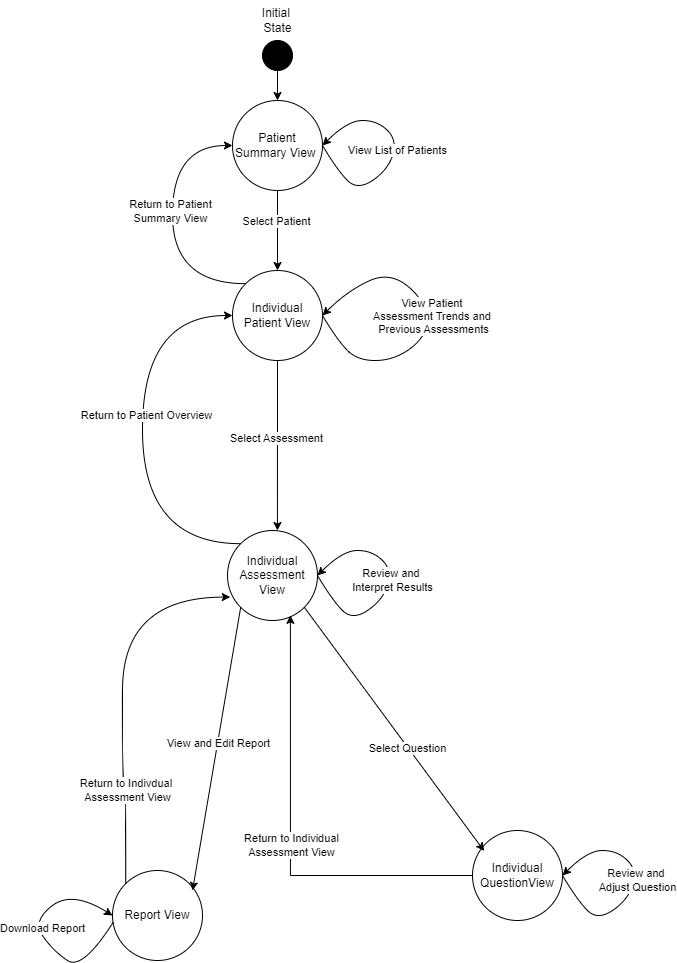
\includegraphics[width=0.75\textwidth]{WorkflowA_State_Diagram.png}
\caption{A finite state machine illustrating the direct analysis workflow (Workflow A) of a clinician when using the MERLS system.}
\label{WorkflowA_State_Diagram} 
\end{center}
\end{figure}

% ============================================================== 
\section{Data Requirements}

\plt{The Data Requirements section describes what information the system must manage.
  It includes the major data entities, their attributes, and the relationships
  between them.  It also includes a data dictionary that defines the meaning of
  each attribute.}

\subsection{Major Data Entities}

\plt{What information must exist for the system to accomplish its goals?}

\plt{For each entity, provide a short explanation.}

\begin{itemize}
\item User
\item Song
\item Session
\item Report
\end{itemize}

\subsection{Data Dictionary}

\plt{For each entity, define all important attributes.}

\begin{longtable}{p{0.20\textwidth} p{0.20\textwidth} p{0.45\textwidth}}
\toprule
Attribute & Type & Description\\
\midrule
user\_id & UUID & Unique identifier\\
email & String & User email address\\
\bottomrule
\caption{Data Dictionary} \label{tab:DataDictionary}
\end{longtable}

\subsection{Privacy and Data Retention}

\plt{Discuss storage, retention, deletion, privacy controls,
 consent, encryption, and compliance requirements.}

TODO

% ============================================================== 
\section{Non-Functional Requirements}

\noindent \begin{itemize}

\refstepcounter{nfrnum}
\item[\textbf{\rthenfrnum}:]
\label{NFR-U1}
  The system shall be intuitive for users with limited technical fluency.
  \\ \textbf{Rationale:} Clinicians’ technical fluency varies, and they have little time to learn new software. An intuitive system shortens the learning curve and avoids the need for formal training.
  \\ \textbf{Fit Criterion:} In usability testing, at least TASK\_SUCCESS\_RATE\% of clinicians with no prior training on the system must complete each core task (e.g., assign a speaker role, view assessment results, add a patient) without assistance within TASK\_TIME minutes.

\refstepcounter{nfrnum}
\item[\textbf{\rthenfrnum}:]
\label{NFR-U2}
  The system shall present all functionality with clear and descriptive labels.
  \\ \textbf{Rationale:} Clinicians work under heavy workloads, and they may be unfamiliar with common software icons. Clear labeling lets them recognize what each function does without guessing.
  \\ \textbf{Fit Criterion:} In usability testing, at least TASK\_SUCCESS\_RATE\% of clinicians must be able to locate and use each core function on their first attempt, relying only on the labels shown on screen and without assistance.

\refstepcounter{nfrnum}
\item[\textbf{\rthenfrnum}:]
\label{NFR-U3}
  The system shall allow clinicians to return to any previously visited stage of their workflow with minimal effort.
  \\ \textbf{Rationale:} Clinicians do not analyze assessments in a straight line. They may go back to review or correct earlier work, so moving between stages should not slow them down.
  \\ \textbf{Fit Criterion:} The clinician must be able to reach any previously visited stage of the workflow from the current page in at most MAX\_NAV\_STEPS navigation steps.

\refstepcounter{nfrnum}
\item[\textbf{\rthenfrnum}:]
\label{NFR-U4}
  The system shall immediately show clinicians the result of each change they submit.
  \\ \textbf{Rationale:} Clinicians edit sensitive patient information; therefore, they need quick confirmation that the system received their change and that it was applied correctly. Without immediate feedback, they cannot tell whether their action was registered, which causes uncertainty and repeated attempts.
  \\ \textbf{Fit Criterion:} The system must display the updated information to the clinician within SYSTEM\_FEEDBACK\_TIME seconds after the clinician submits a change.

\refstepcounter{nfrnum}
\item[\textbf{\rthenfrnum}:]
\label{NFR-S1}
  The system shall only allow a clinician to view the information of patients assigned to them.
  \\ \textbf{Rationale:} Patient assessments are sensitive health information. Access must be limited to the clinician responsible for the patient in order to protect patient privacy and meet data protection obligations.
  \\ \textbf{Fit Criterion:} The system must only list patients assigned to the logged-in clinician and must not allow a clinician to add or access a patient who is in another clinician’s care.

\refstepcounter{nfrnum}
\item[\textbf{\rthenfrnum}:]
\label{NFR-S2}
  The system shall require users to re-enter their credentials after IDLE\_TIMEOUT minutes of inactivity.
  \\ \textbf{Rationale:} Clinicians may leave their workstation unattended, and their accounts contain highly sensitive information. Automatic sign-out prevents unauthorized people from viewing it.
  \\ \textbf{Fit Criterion:} The system must end the user’s session and require credentials before displaying any patient information once the user has been inactive for IDLE\_TIMEOUT minutes.

\refstepcounter{nfrnum}
\item[\textbf{\rthenfrnum}:]
\label{NFR-S3}
  The system shall encrypt patient recordings and transcripts in transit and in storage.
  \\ \textbf{Rationale:} Assessment recordings and transcripts contain private patient information. The annotation service sends video assessments to a third-party transcription service, and the recordings are also kept in the system’s storage. Hence, they must be protected in both places so that anyone who intercepts the data or gains access to the storage cannot read it.
  \\ \textbf{Fit Criterion:} The system must transmit all recordings and transcripts to third-party services using TRANSIT\_ENCRYPTION\_STANDARD and must store them using STORAGE\_ENCRYPTION\_STANDARD.

\refstepcounter{nfrnum}
\item[\textbf{\rthenfrnum}:]
\label{NFR-M1}
  The system shall regularly back up patient information and assessment recordings.
  \\ \textbf{Rationale:} Assessment data is difficult or impossible to recreate, so losing it would waste clinicians’ work and could affect patient care.
  \\ \textbf{Fit Criterion:} The system must back up all patient information and assessment recordings at least every BACKUP\_INTERVAL hours.

\refstepcounter{nfrnum}
\item[\textbf{\rthenfrnum}:]
\label{NFR-P1}
  The system shall only accept video assessments in which the speakers can be clearly seen and heard.
  \\ \textbf{Rationale:} The annotation tool and behavior detection depend on the recording’s quality. Poor audio makes the auto-generated transcript less accurate, whereas poor video quality makes it difficult to detect faces and parent interference. Both instances can lead clinicians to wrong conclusions about a child’s assessment.
  \\ \textbf{Fit Criterion:} The system must only accept submitted assessments where the recording at least meets the minimum video resolution, MIN\_VIDEO\_RESOLUTION, and the minimum audio level, MIN\_AUDIO\_LEVEL. 


\end{itemize}

% ============================================================== 
\section{AI and Machine Learning Requirements}

The system integrates a speech recognition model that was suggested and provided by the capstone team’s supervisors. 
The model was not created by the capstone team. \\

The model used is OpenAI’s Whisper-1, a general-purpose, multilingual automatic speech recognition and translation model. 
It is accessed through an API and takes audio or text as input \citep{OpenAI_Whisper}.

\subsection{Model Inputs}

Individual segments of the assessment’s audio file (.wav), each under 25 MB.

\subsection{Model Outputs}

A JSON object containing the start and end times of each segment, formatted as MM:SS (minutes:seconds), and a text field with the words spoken in the segment.

\subsubsection{Example Output}
\begin{verbatim}
  [
    {
    "start": "00:00",
    "end": "00:05",
    "text": "Recognized words."
    }
  ]
\end{verbatim}

\subsection{Evaluation Metrics}

The model is not currently being evaluated. The annotation tool does, however, let speech clinicians edit transcriptions in chunks, viewing the text next to the audio playback, so incorrect auto-generated transcriptions can be corrected.

The model could be evaluated in the future by comparing the original auto-generated transcriptions against the clinician-edited versions and calculating the word error rate.


\subsection{Known Limitations}

The model’s website describes its performance as average, so the following failure modes are expected when it is used in MERLS \citep{Laumann_Whisper_2022}.
\begin{itemize}
  \item \textbf{Incorrect transcription or translation:} since the model’s overall performance is average, some transcribed or translated text can be wrong. If these errors go unnoticed, clinicians may draw incorrect conclusions about a child’s speech abilities.
  \item \textbf{Incorrect transcription of difficult non-English words: }: the model is known to incorrectly transcribe difficult words in languages other than English. This is concerning for MERLS considering the system is used to assess bilingual children.
  \item \textbf{Uneven performance across different languages:} The model generally performs best on languages with a decent amount of training data, such as Spanish, German, Italian, and English. Transcript accuracy may vary by language, and languages with fewer resources may be transcribed less reliably.
\end{itemize}

Because of these expected failures, MERLS doesn’t treat the model’s output as final. 
Clinicians review the auto-generated transcript against the video playback and correct any errors before relying on it.

% ============================================================== 
\section{Requirements Traceability Matrices}

\begin{longtable}{p{0.15\textwidth} p{0.15\textwidth} p{0.20\textwidth} p{0.20\textwidth}}

\toprule
Stakeholder Req & Use Case & Functional Req \\
\midrule
\srref{SR_Label1} & \ucref{UC_Label1} & \rref{FR_Label1} \\
\bottomrule

\caption{Traceability Between Stakeholder Requirements, Use Cases, and
Functional Requirements} \label{tab:SR2UC2FRtm}
\end{longtable}

\begin{longtable}{p{0.20\textwidth} p{0.20\textwidth}}

\toprule
Functional Req & Nonfunctional Req \\
\midrule
\rref{FR_Label6} & \nfrref{NFR-U2} \\
\rref{FR_Label7} & \nfrref{NFR-U4} \\
\rref{FR_Label8} & \nfrref{NFR-U3} \\
\rref{FR_Label9} & \nfrref{NFR-S1} \\
\rref{FR_Label10} & \nfrref{NFR-U4} \\
\rref{FR_Label22} & \nfrref{NFR-U1} \\
\bottomrule
\caption{Traceability Between Functional and Nonfunctional Requirements}
\label{tab:FR2Rtm}

\end{longtable}

% ============================================================== 

\section{Rationale}

\plt{Provide a rationale for the decisions made in the documentation.  Rationale
should be provided for scope decisions, functional requirements, nonfunctioanl
requirements, data requirements, and AI requirements.  You don't need a
rationale for everything, ust the major decisions that are not obvious.  You
should have traceability to the entities in the document that you are
referencing.}

\section{Likely Changes}    

\noindent \begin{itemize}

\item[LC\refstepcounter{lcnum}\thelcnum\label{LC_meaningfulLabel}:] \plt{Give
    the likely changes, with traceability to the entity that is likely to change.}

\end{itemize}

\section{Unlikely Changes}    

\noindent \begin{itemize}

\item[LC\refstepcounter{lcnum}\thelcnum\label{LC_meaningfulLabel}:] \plt{Give
    the unlikely changes.  The design can assume that the changes listed will
    not occur.}

\end{itemize}

\newpage{}

\section{Appendices}

\subsection{Appendix A: Additional Materials}

This section presents key notes and quotes gathered during the requirements elicitation process for the project.


Several requirements were drawn from research papers describing the system and an experiment conducted by the project supervisor’s team in the United States. 
Although the papers have not yet been released, they describe the entire system and report usability tests with 10 speech clinicians. 
The following highlights the preferences and feedback participants shared while testing the MERLS system and the SAFA annotation tool.

\begin{itemize}
  \item Participant 2 expressed frustration with the amount of time it takes to transcribe assessments: “It would be perfect to have this feature, because doing the annotation part is very time consuming.”
  \item Participant 3 disliked transcribing speech assessments and was enthusiastic about saving time: “when you say that it decreases transcription time, I got very excited about having less time in analyzing speech samples.”
  \item Participant 3 also commented on how BeViz displays results: “I would definitely use the chart/graph/percentages.” This is in regard BeViz in terms of displaying results.
  \item Participant 3 further said they preferred having analysis results summarized as scores, summaries, and patterns rather than as a spreadsheet: “quick and helpful, instead of everything in a spreadsheet.”
  \item Participant 5 suggested what the report should contain: “The whole transcripts for all the [assessment] conversations would be useful to include in the report.”
  \item Participant 5 also raised a concern about data privacy: “the challenge will be the HIPAA, and who has access to data, and how the data could be shared with the parents and the educator.”
  \item Participant 7 appreciated the idea of auto-generated transcripts with human verification in the loop: “we can see a real-time transcription when we play the recording, so that we can do the analysis and give feedback.”
  \item Several clinicians emphasized keeping a human in the loop during the assessment analysis portion of the workflow. For example, Participant 9 stated, “[the system should] allow the clinician to make the final judgment; this is a tool that does not replace our judgment.”
  \item Several clinicians found the system straightforward. For example, participant 10 stated: “I think it’s straightforward. You can see the video recording, originals, [and] place to write notes.”
  \item Clinicians appreciated that the system covered the different aspects of the speech assessment workflow, particularly the ability to move from overall results to an individual question and review its prompt and response. Participant 10 stated, “you have the ‘proof’ there to support your clinical decision and your assessment.”
  \item Participants preferred to have results presented in both English and Mandarin side by side, and to have assessments organized meaningfully by semantics, grammar, and phonology. Participant 10 elaborated: “if you have a feature comparing two languages, side by side in the same graph that would probably be helpful to decide differences vs. disorder.”
\end{itemize}


\subsection{Appendix B: Development Plan}

\plt{This section is optional.  It is used to explain the plan for developing
  the software.  In particular, this section gives a list of the order in which
  the requirements will be implemented.  In the context of a course  this is
  where you can indicate which requirements will be implemented as part of the
  course, and which will be ``faked'' as future work.  This section can be
  organized as a prioritized list of requirements, or it could show the
  requirements that will be implemented for ``phase 1'', ``phase 2'', etc.}

\subsection{Appendix C: Values of Auxiliary Constants}

\plt{Show the values of the symbolic parameters introduced in the report.}

\plt{The definition of the requirements will likely call for SYMBOLIC\_CONSTANTS.
Their values are defined in this section for easy maintenance.}

\plt{The value of FRACTION, for the Maintainability NFR would be given here.}

TODO

\subsection{Appendix D: Generative AI Disclosure}
\subsubsection{AI Tools Used}
\begin{itemize}
  \item Claude Sonnet 5 (Medium)
  \item ChatGPT-5.6 Luna
\end{itemize}

\subsubsection{How and Where Used}
Both models were used in all the sections to do the following:
\begin{itemize}
  \item Check that each written section answered every question asked and met the rubric requirements
  \item Improve the wording, clarity and the flow of written sections
  \item Debug possible LaTeX errors
\end{itemize}

The models were used to do the following in specific sections:
\begin{itemize}
  \item Help brainstorm non-functional requirements in section 8, more specifically for security requirements
  \item Help verify correctness of the FSM diagrams to ensure workflows matched those specified in the research paper in the functional requirements section (Section 6). 
  \item Brainstorm possible non-functional requirements in section 8
\end{itemize}

\subsubsection{Verification of AI-Generated Content}

To verify the output of the LLM, each team member went over their section and presented their work to the group, explaining what they had completed since the previous meeting. 
Each member was able to successfully explain their sections. 
Additionally, before any pull request was approved, a team member who had not written the section reviewed the work to ensure it was cohesive, accurate, and consistent with the rest of the document.\\

The factual content of the documents came from the research of the group members. The writer of each section researched, obtained, and documented all referenced sources. 
After the models suggested wording improvements, the writer re-read the section to confirm that it still conveyed the same point and that the research was not altered.


\subsection{Appendix E: Reflection}

The information in this section will be used to evaluate the team members on the
graduate attribute of Lifelong Learning.  

\input{../Reflection.text}

\input{../SRS_Reflection.text}
\subsection{Nour}
\subsubsection*{Question 1}
Writing the functional requirements was more straightforward than we expected because we had enough resources to understand what our supervisors wanted from the project. 
They provided us with a couple of unreleased research papers that described the system architecture, clinician workflows, including a study they conducted on 10 clinicians to test the TeLaC (now MERLS) platform. 
With this information we were able to create a mental model of the MERLS, SAFA, and BeViz modules and what the purpose for each is. 
Moreover, our supervisors provided us with the GitHub repositories of the annotation tool SAFA and the MERLS system (which is the overall TeleHealth system). 
That let us write requirements that were realistic in how the system behaves and how it should behave once we integrate SAFA. 
Additionally, it made it easier to write use cases that reflected the different clinician workflows detailed in the research papers which are, direct analysis, annotation first analysis, and on-demand refinement. 
These three are the main important workflows and should be enabled by the system very seamlessly. 
Moreover, after speaking with our supervisors, we also learned which areas they are prioritizing and what the main features of the updated system should be. 
This helped us determine what requirements could change and what shouldn’t change in the system. 

\subsubsection*{Question 2}
Creating user personas was my biggest challenge. 
The part of the system our group is working on is mainly for clinicians, so it was hard to identify different types of users, and we were worried the personas would end up looking nearly identical. 
Hence, we created different “types” of clinicians who might use the platform and differentiated them by their work environment and capabilities, such as how heavy their workload is and how comfortable they are with technology. 
This gave us personas that reflect real differences in how the system might be used, which also helped us write non-functional requirements around usability.

Additionally, deciding how detailed each use case should be was also a bit difficult. 
I wasn’t sure where in the workflow each one should start, and simulating the whole workflow from when the clinician enters the system felt like too much. 
It would have repeated the same steps, such as logging in and selecting a patient in every use case. 
Hence, I scoped each use case to a single clinician goal and used the preconditions to set the starting point. 
For example, the clinician is already logged in and has opened a patient’s assessment. 
I also kept the steps focused on what the clinician does and how the system responds, and left out screen-level details, since the interface may change during the redesign.

\subsubsection*{Question 4}
I took SFWRENG 4AL3, the applications of machine learning course. 
It helped me understand the kinds of models our supervisors may have used when building the SAFA tool, and I am comfortable with the machine learning terminology in our documents, such as word error rate and model inputs and outputs. 
Although we did not develop the model and it is not currently being evaluated, I understand how the audio files are segmented and sent to the model for transcription, and I can reason about its known limitations, such as weaker performance on non-English words. 
This is relevant because our users work with bilingual children. The course also taught me why disclosing AI use matters. 
We learned about the negative effects of large language models, including their large carbon footprint, and about the importance of being transparent about how they were used in our documents. 

\subsubsection*{Question 5}
Team management is extremely important for completing the project successfully. 
Our work is split across documents for different milestones, and each member’s section has to fit with the others, so we need a clear picture of who is doing what and when it is due. 
Having good team management lets us stay on top of tasks, stay on the same page, and catch problems early on. 
Moreover, it means regular meetings where each member explains what they have completed since the last one, and discussion regarding the next project steps. 
This is important considering we are balancing the project along with our other courses. 
Furthermore, considering we are building on an existing system with already busy supervisors, we need to communicate regularly with them and record their feedback during meetings. 
Without this, it would be easy for sections to become inconsistent with each other and for team members to be lost or have a different understanding of the project vision and next steps.

Additionally, understanding of how SAFA uses AI to create transcriptions is also important. 
Integrating SAFA into the existing MERLS system is the main focus of our project, so we need to understand how the audio is sent to the model, what the model returns, and where its transcriptions may be wrong, so we can design the system around this.

\subsubsection*{Question 6}
For team management, one approach is keeping a planner or schedule that lists upcoming deadlines, notes, and future meetings. 
It keeps the team on track and helps us balance the project with other courses. 
Another is writing meeting minutes after each meeting. 
Minutes help the team manager see everyone’s tasks and what still needs to be done, so that work is finished on time and with good quality. 
I chose to pursue team management because I have experience with group projects and prefer to know what is happening at all times during a project.

As for understanding how SAFA uses AI, one approach is reading the documentation for the speech recognition model and for SAFA, as well as going through SAFA’s code. 
Another is asking our supervisors to walk the team through how transcriptions are generated and where they tend to fail. 
I will pursue this skill as well, mainly through the documentation and code review, because my machine learning course gave me a background in AI systems and their typical pitfalls, which should help me read the code and judge where the transcriptions may be unreliable.


\newpage

\bibliographystyle {plainnat}
\bibliography {../../refs/References}

\newpage


\end{document}